% \chapter{论文的初始化}
% \label{chp:initialization}

% 在开始撰写学位论文之前,我们建议你首先对你论文的基本信息进行初始化。这部分的工作在main.tex文件中完成。接下来我们将详细介绍各部分的填写方法。注意,下列所有源代码中尖括号{\codefont <...>}里的内容代表你需要填写的文本。

% \section{元数据}

% 元数据部分控制你论文A3封面和中文彩色封面左上角的论文元信息的显示,除固定的学校代码外分为4个部分。下面我们将逐一解释每个部分的填写规则。

% \subsection{分类号}

% 分类号指代中国图书馆分类法 (CLC, Chinese Library Classification)对图书资料的分类编码,请根据你学术论文的内容与分类酌情填写。

% \begin{tcolorbox}
% \begin{lstlisting}[language=TeX]
% \categorynumber{<CLC Code>}
% \end{lstlisting}
% \end{tcolorbox}

% \noindent 举例来说,\textbf{网络安全}的中图法分类号为TN915.08,而\textbf{建筑水利工程}的分类号为F407.9。如对自己研究内容的具体分类不甚确定,可以参阅\href{https://www.clcindex.com/}{相关网站}。

% \subsection{UDC}

% UDC(Universal Decimal Classification)指通用十进制分类法,是国际上规模最大影响最广泛的文献资料分类法。在此部分你需要填写学术论文所属的十进制分类编码。

% \begin{tcolorbox}
% \begin{lstlisting}[language=TeX]
% \UDC{<UDC Code>}
% \end{lstlisting}
% \end{tcolorbox}

% \noindent 举例来说,\textbf{人工智能}的UDC分类号为004.8,而\textbf{凝聚态固态物理学}的分类号为538.9。如对自己研究内容的具体分类不甚确定,可以参阅\href{http://www.udcsummary.info/php/index.php?lang=chi}{相关网站}。

% \subsection{保密级别}

% 在此部分你需要指定你的学术论文所属的保密级别。

% \begin{tcolorbox}
% \begin{lstlisting}[language=TeX]
% \secretlevel{<Secret Level>}
% \end{lstlisting}
% \end{tcolorbox}

% \noindent 一般的,学位论文的保密级别分为公开、内部、秘密和机密四级。具体区别在于:

% \begin{itemize}
%   \item \textbf{公开}:未涉及国家保密范围以及未准备申请专利权或技术转让的一般学术研究;
%   \item \textbf{内部}:未涉及国家保密范围但准备申请专利权或技术转让的在一段时间内不适宜公开的学术研究;
%   \item \textbf{秘密与机密}:涉及国家保密特定密级的科研项目或课题及其衍生的学术研究。
% \end{itemize}

% \noindent 请根据你的论文的具体情况酌情填写。

% \subsection{学号}

% 在此部分你需要填写你的研究生学号。

% \begin{tcolorbox}
% \begin{lstlisting}[language=TeX]
% \studentid{<Student ID>}
% \end{lstlisting}
% \end{tcolorbox}

% \noindent 东南大学的研究生学号一般为6位数字,请注意不要与9位的一卡通号混淆。也请学号为8位数字的本科生同学关闭本文档,出门左转GitHub寻找适合本科生的论文模板。

% \section{论文标题与书脊}

% \subsection{中英文标题}

% 论文标题部分控制你论文的A3封面、中文彩色封面、中文内页封面和英文封面上的标题显示。

% \begin{tcolorbox}
% \begin{lstlisting}[language=TeX]
% \title
%     {弯扭耦合下土木工程复合材料梁的变分渐近模型}
%     {}
%     {Variational Asymptotic Model of Composite Beams Used in Civil Engineering under Bending and Torsion Coupling}
%     {}
% \end{lstlisting}
% \end{tcolorbox}

% \noindent 对论文标题的指定分为4个部分,自上而下分别是中文主标题,中文副标题,英文主标题和英文副标题。对于大多数没有副标题的学位论文,中英文副标题部分可以留空,但请务必不要删去相应的括号。有些论文的中英文标题可能过长,这时你也可以使用副标题位置来实现更加灵活自主的换行。比如上面的示例可以改写成:

% \begin{tcolorbox}
% \begin{lstlisting}[language=TeX]
% \title
%     {弯扭耦合下土木工程复合材料梁}
%     {的变分渐近模型}
%     {Variational Asymptotic Model of Composite Beams Used in Civil}
%     {Engineering under Bending and Torsion Coupling}
% \end{lstlisting}
% \end{tcolorbox}

% \noindent 当你把主标题的后半部分拆分并写到副标题中时,\LaTeX 编译引擎会尝试在你拆分的位置换行。但想要做到这一点需要耐心调整拆分位置,否则如果你的上半部分仍然过长,编译时会被拆分成三行。

% \subsection{论文书脊}

% 论文书脊指出现在A3封面垂直中间部分的文章标题及作者姓名,在论文装订时将被作为书册的书脊。对于大多数学术论文,作者不需要特地显式地声明书脊部分,本模板将会直接利用你的中文标题生成书脊。但如果你的中文标题中出现了英文或其他语言的拉丁字母,直接使用标题生成书脊将会出现图 \ref{fig:2_1} 所显示的问题:

% \begin{figure}[!h]
%   \centering
%     \begin{minipage}[t]{0.3\textwidth}
%     \centering
%     
\includegraphics[width=.3\linewidth]{figures/content/2_1}
%     \caption{错误的书脊渲染}
%     \label{fig:2_1}
%     \end{minipage}
%     \begin{minipage}[t]{0.3\textwidth}
%     \centering
%     
\includegraphics[width=.3\linewidth]{figures/content/2_2}
%     \caption{西文旋转后的书脊渲染}
%     \label{fig:2_2}
%     \end{minipage}
%     \begin{minipage}[t]{0.3\textwidth}
%     \centering
%     
\includegraphics[width=.3\linewidth]{figures/content/2_3}
%     \caption{提升基线后的书脊渲染}
%     \label{fig:2_3}
%     \end{minipage}
% \end{figure}

% \noindent 这时你必须显式地指定书脊的渲染方式。指定的方式很简单,你只需告知编译引擎对标题中的西文字母进行逆时针270$^{\circ}$(即顺时针90$^{\circ}$)旋转即可:

% \begin{tcolorbox}
% \begin{lstlisting}[language=TeX]
% \spine
%     {面向种群的 \rotatebox{270}{Android} 安全风险评估和恶意应用检测}
%     {}
% \end{lstlisting}
% \end{tcolorbox}

% \noindent 请注意,{\codefont $\backslash$rotatebox\{270\}\{\}}前后应该各留一个空格,否则会导致编译错误。和论文标题类似,没有副标题时上述第2个字段可以留空。这样修正后的书脊渲染如图 \ref{fig:2_2} 所示。尽管如此,你仍然能从图 \ref{fig:2_2} 中注意到一些异常。拉丁字母在旋转之后的基线高度比汉字基线高度略低,因此导致书脊中的西文部分看起来总是偏左。解决这一问题,你可以在旋转命令中嵌套基线提升命令,就像这样:

% \begin{tcolorbox}
% \begin{lstlisting}[language=TeX]
% \spine
%   {面向种群的 \rotatebox{270}{\raisebox{2.5pt}{Android}} 安全风险评估和恶意应用检测}
%   {}
% \end{lstlisting}
% \end{tcolorbox}

% 再次修正后的书脊渲染如图 \ref{fig:2_3} 所示,这时你就得到了完美的中西文混排书脊。再次强调,如果你的论文标题中没有中西文混排,请直接删去{\codefont $\backslash$spine}字段。

% \section{作者与导师}

% 该部分用于指定论文的作者与导师姓名。作者字段分为2个部分,分别是作者的中文名及其拉丁文转写:

% \begin{tcolorbox}
% \begin{lstlisting}[language=TeX]
% \author
%     {陈仁营}
%     {CHEN Ren-ying}
% \end{lstlisting}
% \end{tcolorbox}

% \noindent 关于中文姓名转写为英文时的拼写规则,根据《东南大学研究生学位论文格式规定》\cite{seugs2015rule}第一条第二款之要求,有如下规定:

% ~

% \noindent{\color{black!45}
% 中国姓名译为英文时用汉语拼音,按照姓前名后的原则,姓、名均用全名,不宜用缩写。姓全用大写,名的第一个字母大写,名为双中文字时两个字的拼音之间可以不用短划线,但容易引起歧义时必须用短划线。例如“冯长根”译为“FENG Changgen”或“FENG Chang-gen”,而“冯长安”则必须译为“FENG Chang-an”。论文英文封面上的署名也遵守此规定。}

% ~

% 导师字段分为3个部分,分别是导师的中文名、姓名的拉丁文转写以及导师的英文职称,用于显示在英文封面上:

% \begin{tcolorbox}
% \begin{lstlisting}[language=TeX]
% \advisor
%     {张广军}
%     {ZHANG Guang-Jun}
%     {Prof.}
% \end{lstlisting}
% \end{tcolorbox}

% \noindent 对于硕士研究生和博士研究生,导师的职称一般为副教授级及以上。导师为副教授的,职称可以写全称 Associate Professor,也可以写简称 A. Prof.;导师为教授的,可以写全称 Professor或简称Prof.,注意上述简称中的~.不可省略。对于导师职称未达副教授级的特殊情况,比如导师职称为讲师时,请勿在职称处填写Lecturer,此时宜填写Doctor或Dr.以示尊重。

% 一些硕士研究生可能会有副导师,此时可以显式指定副导师的相关信息,具体方法和导师相同:

% \begin{tcolorbox}
% \begin{lstlisting}[language=TeX]
% \coadvisor
%     {程光}
%     {CHENG Guang}
%     {Prof.}
% \end{lstlisting}
% \end{tcolorbox}

% \noindent 没有副导师的研究生学位论文,请删去上述几行。

% \section{答辩信息}

% 答辩信息用于在论文A3封面和中文彩色封面中渲染与研究生论文答辩相关的信息。

% \begin{tcolorbox}
% \begin{lstlisting}[language=TeX]
% \degreetype{工学硕士}{Master of Engineering}
% \major{生物医学工程}
% \submajor{神经信息工程}
% \defenddate{2020年1月20日}
% \authorizedate{2020年1月23日}
% \committeechair{齐康}
% \reviewer{王建国}{韩冬青}
% \department{网络空间安全学院}{School of Cyberspace Security}
% \seuthesisthanks{本文的部分工作受国家自然基金 No. wdnmd666 的支持与帮助,在此表示感谢。}
% \end{lstlisting}
% \end{tcolorbox}

% 其中,{\codefont degreetype}字段用于指定所申请的学位类型与等级。{\codefont major}和{\codefont submajor}字段用于指定研究生攻读的一级和二级学科名称,请依照中华人民共和国教育部一级和二级学科名录进行填写。如果所属专业直接隶属于一级学科,{\codefont submajor}字段可以留空不填。{\codefont defenddate}和{\codefont authorizedate}分别用于指定论文的答辩日期和学位的授予日期,请根据实际情况填写。{\codefont committeechair}和{\codefont reviewer}用于指定论文的答辩委员会主席和论文评阅人。根据《东南大学研究生学位论文格式规定》\cite{seugs2015rule}第二条第一款之要求,有如下规定:

% ~

% \noindent{\color{black!45}
% 论文印刷时尚无法填写的评阅人和答辩委员会主席等栏目待答辩完成后要填写补齐,不要空缺。盲审论文的评阅人处标明“盲审”。}

% ~

% {\codefont department}字段用于指定研究生所属的院系,其中院系的英文名将用于英文封面的生成。学院的正确英文译名请查阅所属学院的官方网站。{\codefont seuthesisthanks}用于在论文的中文内页页脚处对论文所属的项目、赞助的基金课题进行简短的鸣谢。此处不宜书写大段文字,请用简单的一两句话对相关组织或机构表示感谢,对其他个人的感谢请在文尾的致谢部分进行。没有相关赞助的学位论文请直接删去该字段。

% \section{模板参数}

% 你有可能已经注意到了在main.tex文件中引入模板类的命令里包含了若干模板参数:

% \begin{tcolorbox}
% \begin{lstlisting}[language=TeX]
% \documentclass[algorithmlist,figurelist,tablelist,nomlist]{seumasterthesis}
% \end{lstlisting}
% \end{tcolorbox}

% \noindent 即{\codefont documentclass}命令后的中括号里的几个参数。这些参数用于控制条件编译以及在论文渲染时向模板类提供额外的信息。本节将会介绍本模板提供的模板参数及其具体含义。

% \subsection{链接着色}

% 本模板通过使用hyperref宏包来提供索引和链接跳转功能。相信你已经注意到了,本模板所渲染出的PDF文档中的所有图片、表格、公式、算法和参考文献索引都被着色高亮,且可以通过点击跳转到原引位置。该功能便于读者在阅读电子文档时快速定位相应索引的位置,但是着色高亮的链接在论文付梓时可能会影响到印刷效果。因此,本模板提供了针对链接着色的模板参数。通过在模板参数列表中添加{\codefont nocolorlinks}参数,模板所渲染出的PDF文档中的所有文献索引都将被取消着色,以便论文的正式印刷。

% \subsection{图表、算法及术语目录}

% 根据不同院系和专业的具体情况,硕士研究生学位论文可能并不需要图表、算法或术语目录中的一项或多项。尽管本模板默认会渲染出上述的所有目录,但是我们也提供了相应的模板参数来灵活控制这些目录的渲染。如果你在模板参数列表中显式指定{\codefont figurelist},代表你希望在论文编译时在章节目录后添加图片目录;类似的,{\codefont tablelist}显式指定了表格目录的需求,{\codefont nomlist}指定了术语表,而{\codefont algorithmlist}指定了算法目录。需要注意的是,你并不需要关注这几个模板参数在参数表中的位置或顺序,具体目录的编译和渲染仍然会依照《东南大学研究生学位论文格式规定》\cite{seugs2015rule}第一条中所规定的顺序进行。

% \subsection{硕士类型}

% 本模板同时支持学术型硕士研究生和专业型硕士研究生。当不添加任何模板参数时,该模板将默认渲染为学术型硕士研究生学位论文;而当在模板参数列表中显式指定{\codefont engineer}时,该模板将渲染为专业型硕士研究生学位论文。专业型与学术型硕士研究生学位论文的区别主要在于以下三点:
% \begin{enumerate}
%     \item A3 大封面和中文彩色封面的\textbf{标题}。学术型硕士为《硕士学位论文》,专业型硕士为《工程硕士学位论文》。需要注意的是,中文内页封面的标题在两种类型的硕士研究生学位论文中均为《硕士学位论文》。
%     \item A3 大封面和中文彩色封面的\textbf{学位论文形式}。专业型硕士研究生需要注明学位论文的研究形式,如应用研究、基础研究或综合研究。因此专业型硕士研究生需要填写main.tex文件中的{\codefont engthesistype}字段,学术型硕士研究生则可以忽略该字段。
%     \item A3 大封面和中文彩色封面的\textbf{学科名称}。学术型硕士研究生学位论文需要在答辩信息列表中填写一级和二级学科名称,而专业型硕士研究生需要填写的则是工程领域名称和研究方向。因此专业型硕士研究生需要在main.tex文件的{\codefont major}字段填写自己的工程领域名称,在{\codefont submajor}字段填写自己的研究方向。
% \end{enumerate}


\chapter{无线密钥生成系统的理论基础}

本章节主要介绍无线密钥生成系统的理论基础。无线密钥生成系统的本质是利用无线信道的短时互易性、时空唯一性进行密钥生成的工作,在信道探测之后,量化生成的CSI,并进一步调和和隐私放大。另外本章介绍了系统生成密钥的评估标准,通过CSI相关性、信道随机性、密钥随机性和信息泄漏率等四个方面评估系统生成密钥的可靠性和安全性。

\section{无线信道特性}

\subsection{无线信道的短时互易性}

在TDD系统的上下行链路中,假设通信双方Alice和Bob以及窃听者Eve。在相干时间内,Alice和Bob互相发射的信号经过相同的信道衰落,因此由此估计出的信道具有互易性\cite{ye2010information}\cite{azimi2007robust}。

在图\ref{wireless-channel}中,Alice和Bob之间上下行链路的频率响应分别为$H_{ab}(t)$和$H_{ba}(t)$,相干时间内有$H_{ab}(t) = H_{ba}(t)$。假设在一次信道探测过程中,探测时隙为$\Delta t$,相干时间$\tau$内,Alice和Bob分别测量信道为$\tilde{H_{ba}(t)}$和$\tilde{H_{ab}(t)}$,当$ \Delta t < \tau $时有,

\begin{equation}
    H_{ba}(t) \approx H_{ab}(t + \Delta t)
\end{equation}

即双方探测的信道是近似相同的,因此通信双方可以通过利用无线信道的短时互易性来探测信道,进而结合其他协议生成相同的一致密钥。

同时,由于射频端的非线性特性、信道估计引入的误差、信道的时变性等因素\cite{guillaud2005practical},通信双方对信道的探测结果会有波动性差异:

\begin{itemize}
    \item 器件非线性。射频器件的非线性会导致I/Q路不平衡,如图\ref{iq_imbalance}所示,IQ不平衡会直接影响信号的发射和接收。在TDD系统中,收发两端的IQ不平衡会给上下行信道估计的互易性带来损失。
    \item 信道时变性。在相干时间内,无线信道具有短时互易性。但是由于无线信道的时变性,当双方探测信道的时隙超过信道相干时间,上下行信道估计结果会出现一定差异。
    \item 信道估计引入的误差。在基于导频的信号估计中,通过接收的导频信号和发射的导频信号做数学运算估计信道的频率响应,算法原理是通过最小化均方误差来估计信道,因此算法本身具有一定误差。
    \item 其他。另外,还有上下行链路的加性噪声也会对接收的信号有加性影响,不同频率子载波也会导致上行链路的差异等等。
\end{itemize}

\begin{figure}[htbp!]
    \centering 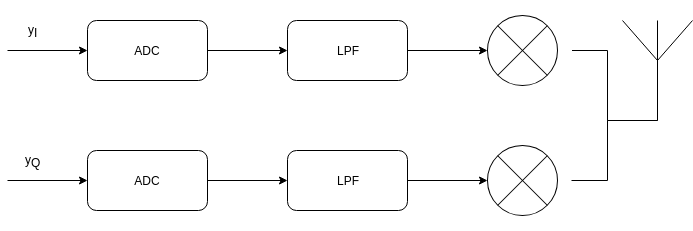
\includegraphics[width=0.6\textwidth]{images/iq_imbalance} 
    \caption{发射机存在的IO不平衡}
    \label{iq_imbalance}
\end{figure}


目前已经有相关工作研究如何对信道互易性的损失进行补偿,比如信道预测技术对信道互易性进行补偿,其原理是利用信道探测数据本身对未来时间的信道数据做出预测\cite{heidari2010adaptive}。另外基于信道互易性的MIMO预处理技术也可以一定程度上提高信道互易性,进而提高密钥一致性。针对IQ不平衡致使的信道互易性损失,可以估计系统中的不平衡参数,使相邻子载波的均方误差最小\cite{tubbax2005compensation}。

\subsection{无线信道的时空唯一性}

\begin{figure}[htbp!]
    \centering 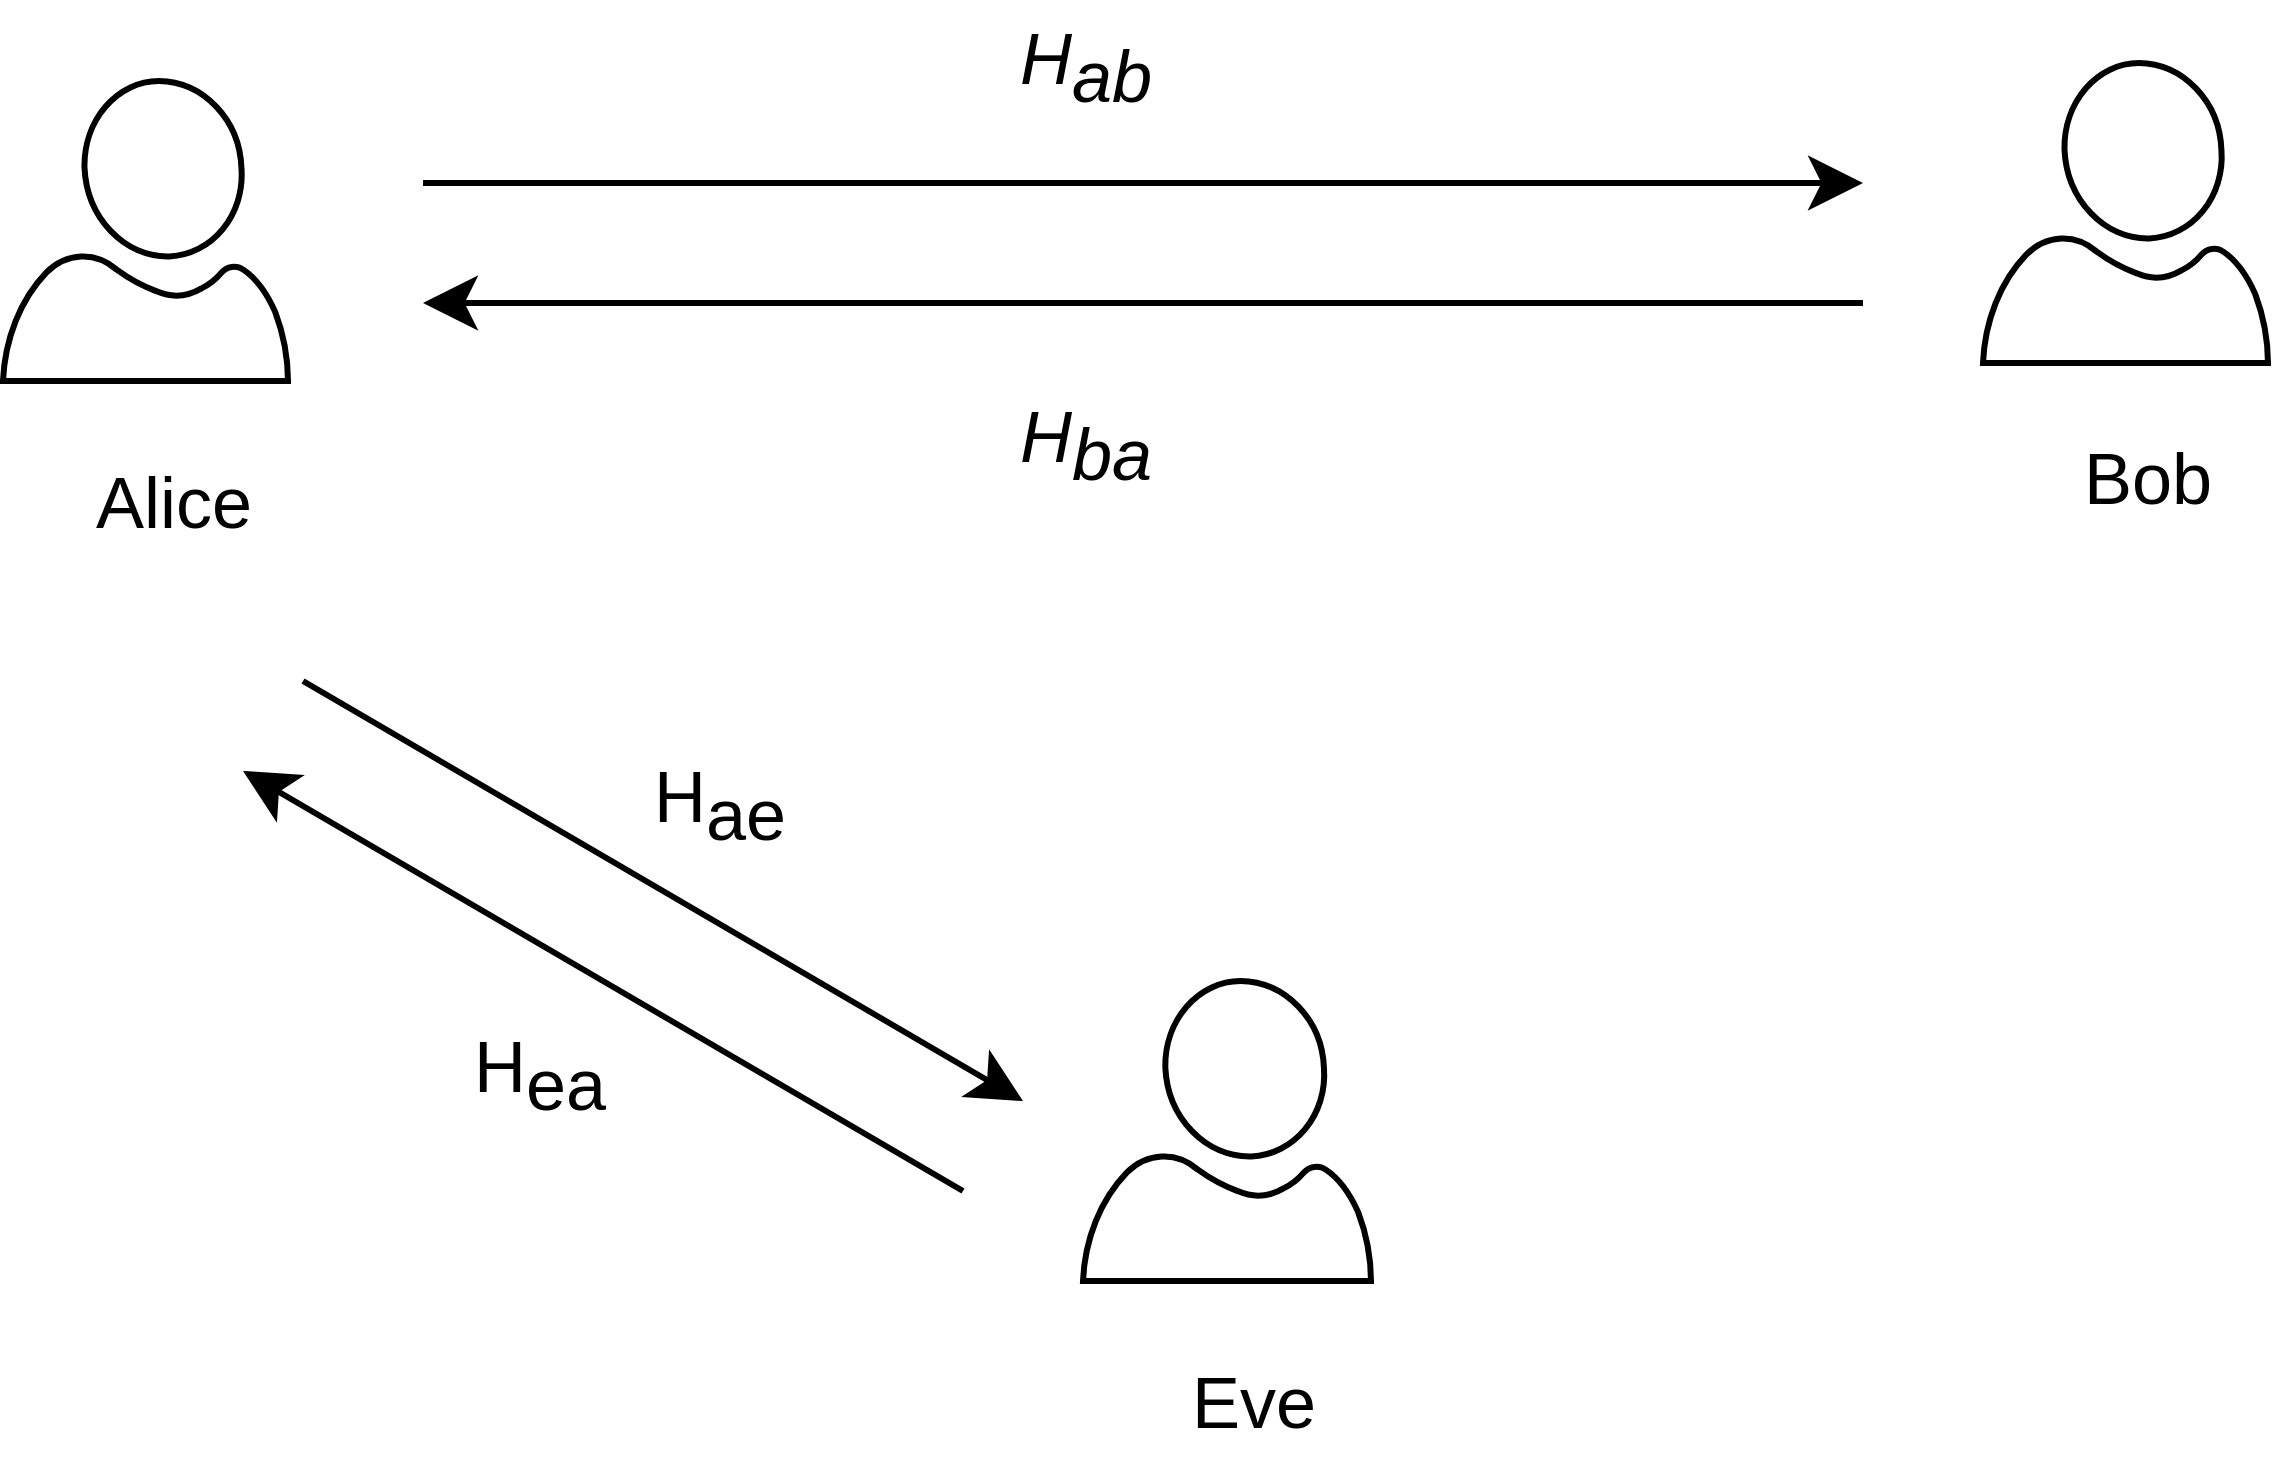
\includegraphics[width=0.6\textwidth]{images/channel} 
    \caption{无线通信信道}
    \label{wireless-channel}
\end{figure}

如图\ref{wireless-channel}所示,在某时刻t,通信双方Alice和Bob互相发射导频信号,在相干时间内,经管相同的多径信道衰落,对于窃听者Eve来说,无论是窃听来自Alice还是Bob的发射信号,其信道衰落都不同于Alice和Bob之间的信道衰落。在相干距离d(半波长)以外,Eve接收信号经历的多径衰落与Bob接收信号的多径衰落不再相关。除非攻击者在物理空间上靠近任意合法通信双方,否则无法分析出通信双方的CSI\cite{sasaoka2009secret}。

\subsection{无线信道的时变特性}

% 参考 3.1.1

信道衰落分为两类,大尺度衰落和小尺度衰落。大尺度衰落包括路径损耗和阴影损耗,在长距离传输(上百米)中,信号强度会发生变化。路径损耗指空间传播中电磁波的损耗,阴影损耗指在电磁波在传输过程中,受到遮挡物影响产生阴影效应,导致场强变化。通常用自由空间模型、Hata-Okumura,模型等来描述大尺度衰落。在大尺度衰落下,无线信道的特征提取主要是基于其接收信号强度(RSSI)的变化。由于不同位置下的阴影效应,导致接收信号强度产生了变化。

小尺度衰落通常反应在短距离范围内信号幅值的变化中,通常符合瑞利分布、莱斯分布,小尺度衰落分为快衰落信道和慢衰落信道,快衰落信道又分为空间选择性快衰落信道、时间选择性快衰落信道、频率选择性快衰落信道。小尺度衰落反应无线信道的多径和时变,在无线通信中,通信双方之间信号经过的物理路径比较复杂,会收到多径的影响,可以将多径衰落信道建模成时变脉冲有限响应滤波器(FIR)\cite{liu2012exploiting},即,

\begin{equation}
    h(\tau, t) = \sum_{l = 1}^{N(t)} a_k(t) \sigma(\tau - \tau_k(t))
\end{equation}

其中,t时刻,多径分量个数为$N(t)$,$a_k(t)$表示t时刻第l条路径信号幅度,$\tau_k(t)$表示t时刻第l条路径的延迟。

当无线信道的多径时延可以被信道测量信号所区分时,该测量得到的无线信道特征将主要反映了无线信道的多径变化的结果。当接收者位置发生改变时,其接收信号的多径分布以及不同多径受位置变化影响产生的相位改变将会导致无线信道的状态信息(CSI)的显著变化。


\section{密钥生成流程}

本文基于无线信道密钥生成技术设计的系统主要分为四个阶段,信道探测、特征量化、信息调和,整体架构如图\ref{whole_structure}所示。其中,Alice和Bob是合法通信双方,Eve是第三方窃听者。信道探测阶段是无线信道传输导频信号,信息调和阶段是通过公共信道传输调和信息。

\begin{figure}[htbp!]
    \centering 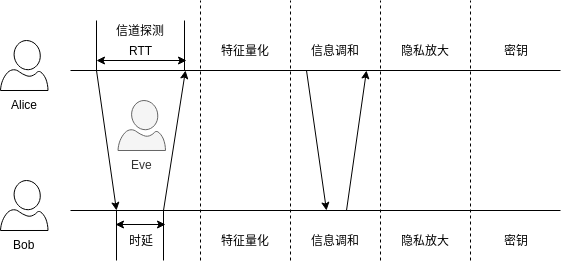
\includegraphics[width=0.9\textwidth]{images/whole_structure} 
    \caption{无线密钥生成流程的整体架构}
    \label{whole_structure}
\end{figure}

\subsection{信道探测}

在一个单入单出线性系统中,设脉冲响应函数为$g(k)$,根据维纳-霍夫方程的离散形式,发射信号$x(k))$和$y(k)$之间的相关函数为,

\begin{equation}
    R_{xy}(\tau)  = \sum_{j=0}^{\infty} g(j) R_x(\tau-j)\Delta t
\end{equation}

同时,M序列的自相关函数为,

\begin{equation} \label{m_self}
    R_m(\tau) = \left\{
  \begin{aligned}
  &1, &\tau = 0, N, 2N, ... \\
  &-\frac{1}{N}, &wherelse \\
  \end{aligned}
  \right.
\end{equation}

因此,当发射信号x(k)为M序列时,即$x(k) = m(k)$时,有,

\begin{equation}
    R_{ym}(k) = \sum_{j=0}^{N-1} \tilde{g}(j)R_m(k-j)\Delta t
\end{equation}
\begin{equation}
    R_{ym}(k) = \frac{(N+1)\Delta t}{N} \tilde{g}(k) - \frac{\Delta t}{N} \sum_{j=0}^{N-1} \tilde{g}(j)
\end{equation}
  
\begin{equation}\label{eq1}
    \tilde{g}(k) = \frac{N}{(N+1)\Delta t} [R_{ym}(k) + c]
\end{equation}

其中,

\begin{equation}
  R_{ym}(k) = \frac{1}{N}\sum_{j=0}^{N-1}m(j-k)y(j)
\end{equation}

工程上,

\begin{equation}
  c=-R_{ym}(N_P - 1)
\end{equation}
  
在TDD/FDD系统中,用户Alice和Bob互相发送导频信号帧$m(t)$作为导频信号。设$h_{ab}$代表Alice到Bob信道的频率响应,$h_{ba}$代表Bob到Alice信道的频率响应。那么,

Alice检测的时域信号为,

\begin{equation}
    y_{ba}(t) = m(t) * h_{ba}(t) + n_{ba}(t) 
\end{equation}

Bob检测的时域信号为,

\begin{equation}
    y_{ab}(t) = m(t) * h_{ab}(t) + n_{ba}(t)    
\end{equation}

因此Bob通过式(\ref{eq1})估计信道,

\begin{equation}
    \tilde{h}_{ab}(k) = a\sum_{j=0}^{N-1}m(j-k)y_{ab}(j)
\end{equation}
  
同理,Alice通过式(\ref{eq1})估计信道,
  
\begin{equation}
    \tilde{h}_{ba}(k) = a\sum_{j=0}^{N-1}m(j-k)y_{ba}(j)
\end{equation}
  
其中,a为常数,

\begin{equation}
    a = \frac{2-N_p}{(N + 1)\Delta t}
\end{equation}

\subsection{预处理}

在步骤信道探测中,通信双方分别通过导频信号估计探测时隙$\tau$内的脉冲响应$\tilde{h}_{ba}$和$\tilde{h}_{ab}$,并进行快速傅里叶变换得到信道频率响应$\tilde{H}_{ba}$和$\tilde{H}_{ab}$。由于在探测过程中,无线信道测量结果会受到环境噪声、射频器件的非线性等因素影响,因此通常会进一步预处理来提高信道的互易性和消除数据冗余。

\begin{equation}
    \tilde{H}_{ba} = Pre(FFT(\tilde{h}_{ba}))
\end{equation}
\begin{equation}
    \tilde{H}_{ab} = Pre(FFT(\tilde{h}_{ab}))
\end{equation}

其中,$Pre$表示预处理函数,$FFT$表示快速傅里叶变换。

\subsection{特征量化}

目前有多种量化策略,常用的有单门限量化、多门限量化、自适应门限量化等。

文献\citen{aono2005wireless}采用如图\ref{single_quantization}所示的单门限量化,量化阈值取RSSI(Radio Signal Strength Indicator)平均值,可以带来比较高的密钥一致率,但是测量值在阈值附近时容易量化错误,并且由于量化精度不高,在信道变化缓慢时,生成密钥容易出现大量连续0比特和1比特长串。

\begin{figure}[htbp]
    \centering
    \begin{minipage}[t]{0.48\textwidth}
        \centering
        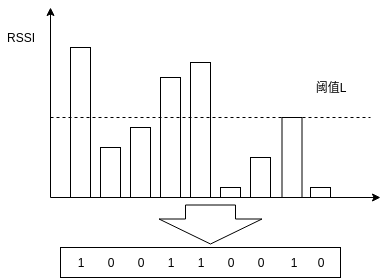
\includegraphics[width=6cm]{images/single_quantization}
        \caption{单门限量化}
        \label{single_quantization}
    \end{minipage}
    \begin{minipage}[t]{0.48\textwidth}
        \centering
        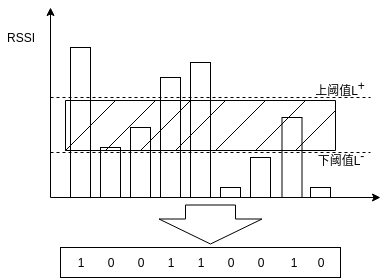
\includegraphics[width=6cm]{images/two_quantization}
        \caption{双门限量化}
        \label{two_quantization}
    \end{minipage}
\end{figure}

文献\citen{mathur2008radio}采用如图\ref{two_quantization}所示双门限量化,将门限$L^+$和$L^-$之间的值舍弃,将$L^+$以上的值量化为1,将$L^-$以下的值量化为0,通信双方会在公共信道上交互传输未舍弃比特位的索引信息,因此第三方窃听者只有可能得知哪些比特被使用而无法得知被量化成0还是1,但是会降低密钥生成速率。


文献\citen{patwari2009high}通过多次测量表明双门限量化每次会丢失5\%至27\%的比特数,并提出多比特自适应量化方法。文献\citen{yasukawa2008secret}使用多级量化,先将RSSI根据大小排序,然后分割成等间隔的$N = 2^m$块,m是量化比特数,并且通常$N \leq log_2^{maxValue}$,这样每个量化阶值的出现率是相同的。

通常多比特量化之后,会进一步编码成对应阶数格雷码。格雷码的特性是,相邻位置的格雷码只有一个位置的比特不同,因此使用格雷码可以提高通信双方的密钥一致率。无论是上述哪种量化方法,都避免不了密钥生成率和密钥一致性之间的矛盾。量化阶数越高,量化比特数越多,密钥生成率越高,但误差影响较大,密钥一致率降低;量化阶数越低,量化比特数越少,密钥一致率越高,但是密钥生成速率越低。

本文使用均匀量化的方法。在一次密钥生成过程中,Alice和Bob分别探测信道、预处理得到CSI。先对CSI降采样,以降低密钥泄漏率\cite{linning2019investigation}。同时,量化可以降低噪声的影响\cite{wang2015survey}。设量化时CSI最大值为$m_{max}$,量化阶数为R,量化前的值为m,量化后的值为q,将CSI归一化后按照式\ref{quantization_formula}均匀量化,得到离散的采样值,采样值对应比特数即量化阶数,本文量化阶数为3。密钥的生成速率与量化阶数成正比,通信双方的密钥一致率与量化阶数成反比。因此可以根据信噪比去调整量化阶数以得到较为均衡的密钥生成速率与一致率。量化之后的采样值需要进一步格雷编码降低密钥的不一致率。然后进行8b10b编码,过程如图\ref{quantization}所示。

\begin{equation} \label{quantization_formula}
    q = \frac{2^R * m}{m_{max}}
\end{equation}

\begin{figure}
    \centering
    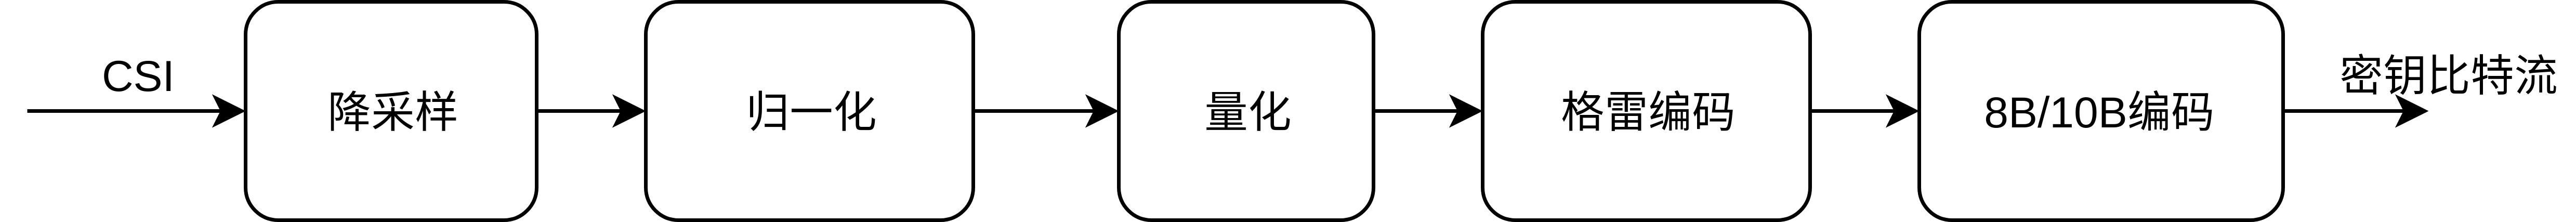
\includegraphics[width=0.9\textwidth]{images/quantization}
    \caption{量化}{} % Quantization.
    \label{quantization}
\end{figure}

\subsection{信息调和}

信息调和是在公共信道对不完全一致的密钥信息协商。由于短时信道互易性,所以通信双方分别通过上述步骤提取出的密钥是近似的,但是由于信道在探测的时隙内发生变化、环境中的干扰以及硬件指纹等各种因素,双方提取出的密钥又是不完全一致的。因此需要进一步调和。

信息调和通常基于Caseade协议\cite{Kitano2007A}或者纠错编码,比如 Turbo 码,BCD 码,LDPC 码等\cite{peng2018securing}。本文使用两种方式调和生成密钥。假设通信双方Alice和Bob,量化之后提取的比特字符串为$key1$和$key2$。

如果通过CRC校验码去除不一致比特,那么Alice将比特字符串$key1$分组并计算CRC校验码,将冗余部分码字发送给Bob。Bob进行同样分组,并根据Alice发送过来的冗余部分码字去除不一致的组。Bob再将检验结果回发给Alice,Alice根据校验结果去除不一致的组。最终双方可以得到一致的会话密钥。使用CRC校验码的调和过程如图\ref{crc}所示。

\begin{figure}
    \centering
    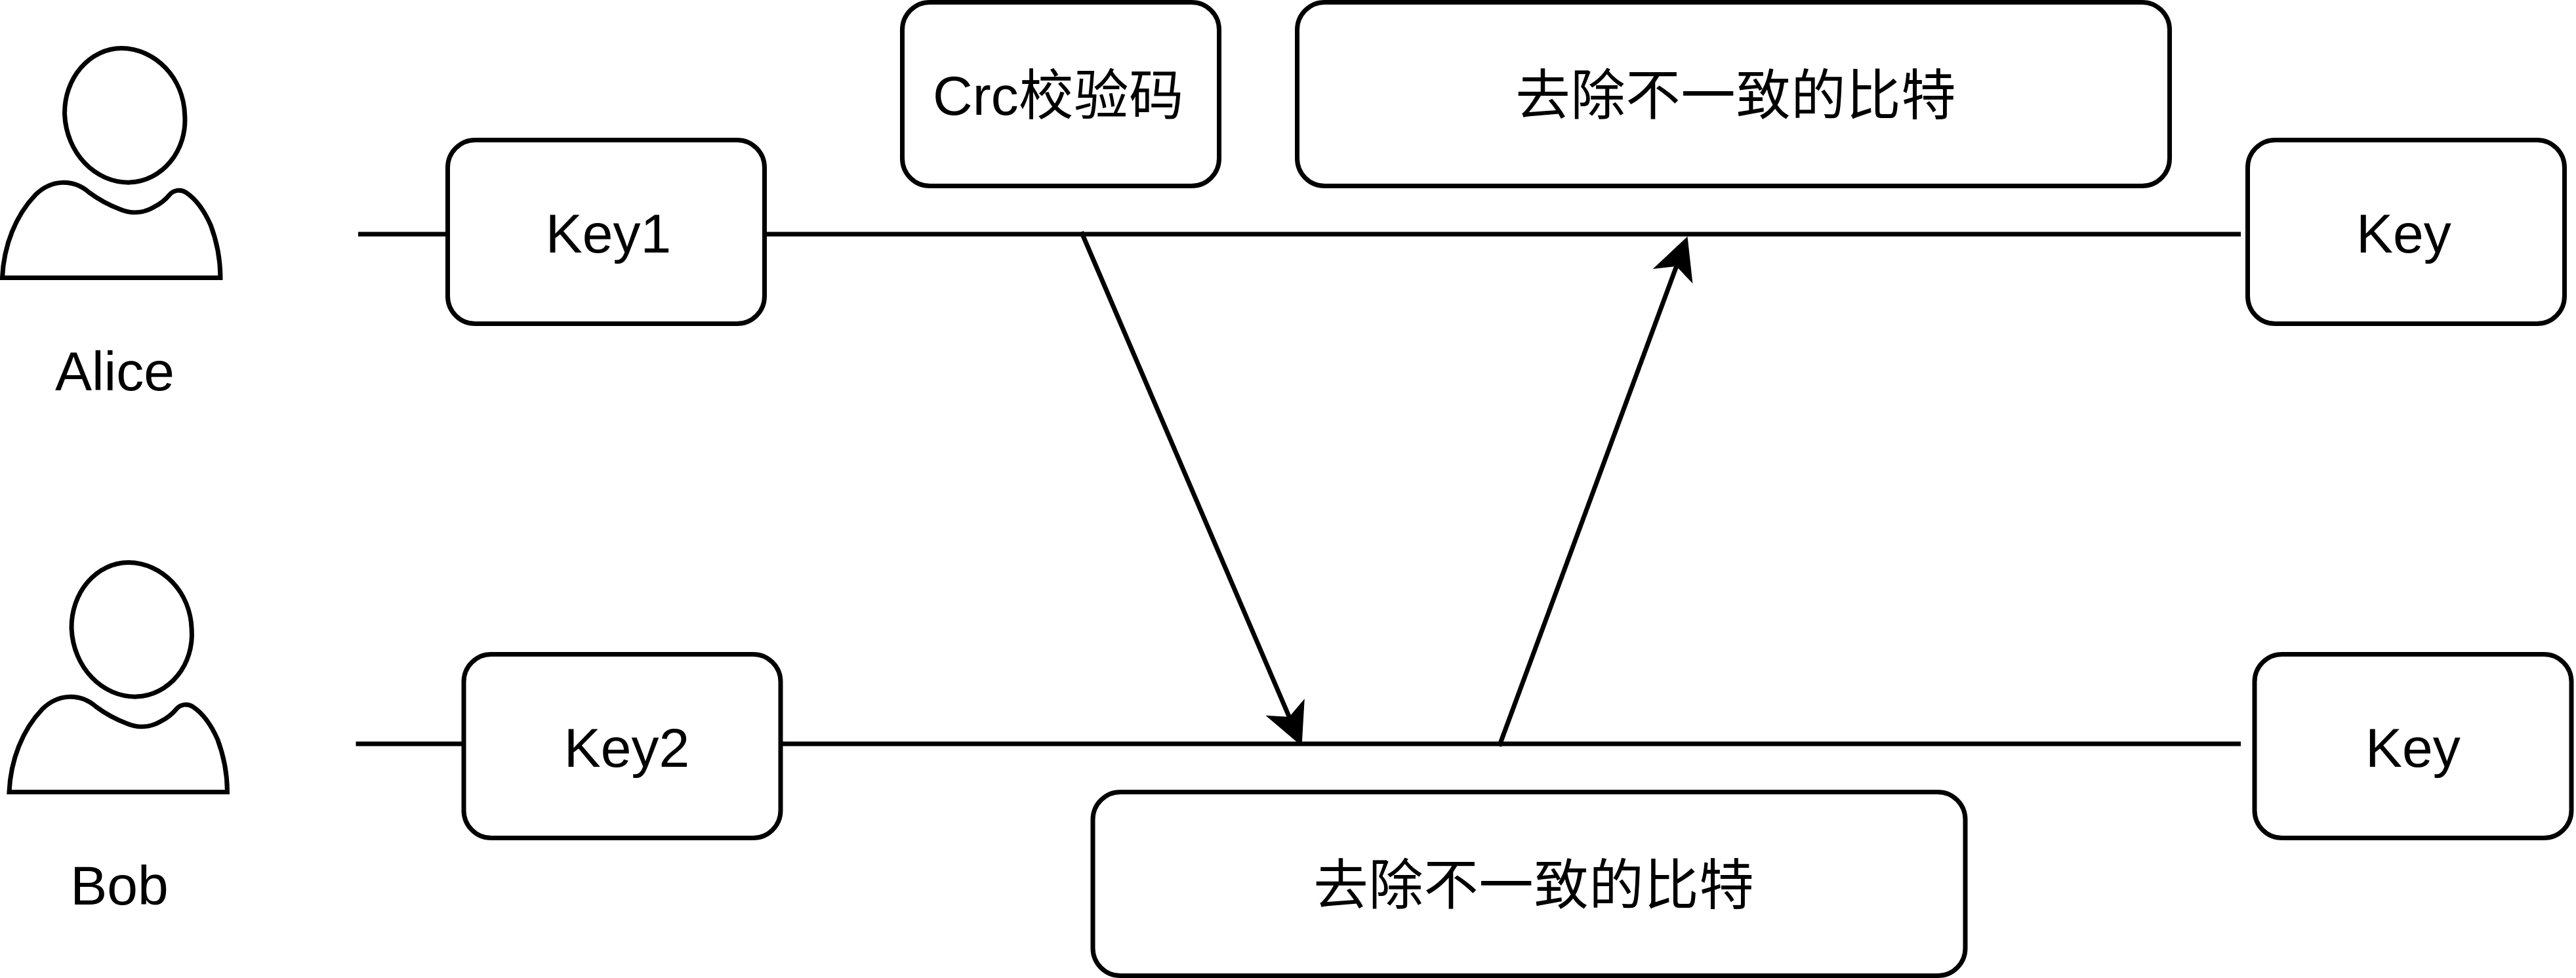
\includegraphics[width=0.9\textwidth]{images/crc}
    \caption{信息调和}{} % Crc Reconciliation
    \label{crc}
\end{figure}

% todo 纠错解码着一块还可以写的更加详细一点
除了通过CRC校验码去除不一致比特,Alice先将会话密钥进行纠错编码,再和key1异或,然后发送给Bob,Bob再次和key2异或,之后通过纠错解码器纠正错误比特位得到会话密钥key'。使用纠错码的过程如图\ref{error_correcting_code}所示。

\begin{figure}
    \centering
    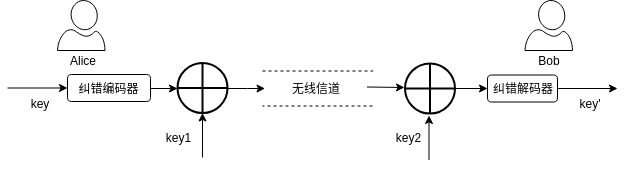
\includegraphics[width=0.9\textwidth]{images/error_correcting_code}
    \caption{纠错码}{} % Crc Reconciliation
    \label{error_correcting_code}
\end{figure}

% TODO
\subsection{隐私放大}

由于信道探测阶段和信息调和阶段,通信双方之间交互的中间信息对外界全部透明,中间信息中可能分析出密钥,因此为了防止密钥信息被泄露,所以需要进一步隐私放大。隐私放大是允许双方从窃听者拥有部分信息的公共随机变量中提取密钥的过程。双方一般对窃听者的信息一无所知,只知道它满足一定的约束条件。隐私放大使得密钥协商成为可能,在密码学领域有着广泛应用\cite{vernam1926cipher}。

假设Alice和Bob拥有变量W(n比特),窃听则Eve从变量W中窃听到变量V(t比特,t < n且比特位随机),并且满足约束$ I(W;V) \leq t $,那么Alice和Bob可以仍然协商出Eve无法得知的$n-t$比特的密钥\cite{bennett1988privacy}。通常可以使用Hash函数来完成隐私放大\cite{wegman1981new},其将任意长度的字符串映射到一个固定长度的字符串。

\section{无线信道密钥的评估标准}

本文为评估无线密钥生成系统性能,通过CSI相关性、信道随机性、密钥随机性和信息泄漏率等四个方面评估系统生成密钥的可靠性和安全性。

\subsection{CSI相关性}

本文通过皮尔逊相关系数计算CSI相关性,假设通信系统中,合法通信双方Alice和Bob信道探测结果为$\tilde{H}_{ba}$和$\tilde{H}_{ab}$,窃听者Eve探测结果为$\tilde{H}_{ae}$。

那么Alice和Bob之间CSI相关性为,

\begin{equation}\label{equation_corr_ab}
    Reprocity_{ab, ba} = \frac{E[(\tilde{H}_{ab}-\mu_{\tilde{H}_{ab}})(\tilde{H}_{ba}-\mu_{\tilde{H}_{ba}})]}{\sigma_{\tilde{H}_{ab}}\sigma_{\tilde{H}_{ba}}}
\end{equation}

为研究Eve窃听的CSI结果与合法信道的CSI结果的差异,计算Eve的CSI和Alice的CSI相关性,

\begin{equation}\label{equation_corr_ae}
    Reprocity_{ab, ae} = \frac{E[(\tilde{H}_{ab}-\mu_{\tilde{H}_{ab}})(\tilde{H}_{ae}-\mu_{\tilde{H}_{ae}})]}{\sigma_{\tilde{H}_{ab}}\sigma_{\tilde{H}_{ae}}}
\end{equation}

其中,$\sigma_{\{.\}}$表示标准差,$E\{\cdot\}$表示期望。

理论上,在相干距离之外,

\begin{equation}
    Reprocity_{ab, ae} < Reprocity_{ab, ba}
\end{equation}

$Reprocity_{ab, ba}$越大表明合法通信双方信道互易性越好,CSI相关性越高,密钥一致率越高。$Reprocity_{ab, ba}$较低的原因可能是通信双方硬件指纹差异、信道环境糟糕等,可以使用一些预处理算法弥补互易性的损失。

$Reprocity_{ab, ae}$越小表明第三方可以窃听的信息越少,CSI相关性越低,密钥泄露更少。在相干距离(通常是半波长)以外,由于导频信号经过不同的信道衰落,因此Eve估计得到的CSI与合法信道的CSI相关性较低。在相干距离以内,由于物理距离上接近,Eve估计的CSI相关性较高,但是在实际环境中,窃听者无法如此靠近合法通信参与者。

\subsection{信息泄露率}

本文设计的密钥生成系统中,在信道探测、信息调和阶段,对第三方来说是完全透明的\cite{sahin2016secure}。设Alice、Bob和Eve对信道探测为$H_A$、$H_B$和$H_E$。则A和B之间信道的互信息为,

\begin{equation}
    I_k = I(H_A; H_B) = log_2^{\frac{\left|R_{AA}\right|\left|R_{BB}\right|}{\left|R_{AB}\right|}}
\end{equation}

其中, $\left|R_{xy}\right| = E\{H_x H_y^H\}$表示协方差系数。

存在eve时,alice和bob之间的互信息量为, 

\begin{equation}
  I_{sk} = I(H_A; H_B | H_E) = log_2^{\frac{\left|R_{AE}\right|\left|R_{BE}\right|}{\left|R_{EE}\right|\left|R_{ABE}\right|}}
\end{equation}

通过$I_{sk}$与$I_k$的比例来评估信息未泄露的比率,

\begin{equation} \label{safe_rate_equation}
  \eta = I_{sk} / I_k
\end{equation}

\subsection{随机性评估}

本文既评估了系统运行过程中的CSI随机性,也测试了生成密钥的随机性。

\subsubsection{CSI随机性}

CSI的随机性既有时域的变化,也有频域的变化。为了衡量CSI的随机性,本文采集了不同场景下的多组CSI,计算多组CSI的图像熵,用来衡量CSI的随机性。

使用二维快速傅里叶变换(2D-FFT)的图像熵来表征信道的随机性。设计算得到的多组CSI归一化之后为矩阵$C_{MxN}$,M为CSI长度,N为采集的CSI组数。$C(x, y)$表示第i行第j列的值,那么对其做2D-FFT的矩阵为,

\begin{equation}
  F(u, v) = \frac{1}{MN}\sum_{x=0}^{M-1}\sum_{y=0}^{N-1} C(x,y) e^{-j2\pi(\frac{xu}{M}+\frac{yv}{N})}
\end{equation}


为了缩小差距,将$F$取In函数得到$L$,

\begin{equation}
  L(u, v) = log_e^{F(u, v)}
\end{equation}

再归一化到[0, 1]范围内得到,

\begin{equation}
  I(u, v) = \frac{L(u, v) - min{L}}{max(L) - min(L)}
\end{equation}

将[0, 1]区间分割成256等份,统计I(u, v)在各个区间的概率,计算I(u, v)的熵,

\begin{equation} \label{entropy_fft2d_equation}
  H(u, v) = -\sum_{i=1}^{256} p_i log_2^{p_i}
\end{equation}

\subsubsection{密钥随机性}

本文使用NIST(National Institute of Standards and Technology,NIST)随机性测试来评估密钥的随机性\cite{bassham2010statistical}。NIST随机性测试通过多个维度测试密钥的随机性\cite{zaman2012review}。NIST官网包含了16项统计测试,每项测试会对给定比特序列做在随机性假设下的卡方检验,其将$\chi^2$值转换为随机性概率,即程序中的P值,表示随机性的可能性大小。表\ref{NIST-schemes}为NIST随机性测试的15项测试手段。如果P值大于0.01,则表示比特序列是随机的。

% 参考

\begin{table}[]
    \centering
    \begin{tabular}{p{70pt}p{70pt}p{200pt}p{100pt}}
    \hline
    方法 & 参数要求 & 原理 & 不通过原因 \\ \hline
    频数检验 & N $\geq$ 100bits & 序列中1和0数目是否相近 & 说明1和0数目相差过多  \\ \hline
    块内频数检验 & N $\geq$ 100bits 子块 M > 0.01N & M位子块中1的个数是否接近m/2 & 至少某一个子块0、1比例不均衡 \\ \hline
    游程检验 & N $\geq$ 100bits 设定$\tau = \frac{2}{\sqrt{n}}$,用于判定是否频数检验 & 检验不同长度的游程总数是否符合随机序列的期望值 & 说明游程综述过大或者过小,即,序列中元素变化过快或者过慢  \\ \hline
    块内最长游程检验 &  & 检验序列中各个等长子序列中最长1游程的长度是否符合随机序列的期望值 & 检验序列中有太多的(成簇的)1 \\ \hline
    二元矩阵秩检验 & N $\geq$ 38MQ,行列M=Q=32 & 由检验序列的给定长度子序列构成序列,检验构造矩阵行或列之间的线性独立性 & 秩分布与相应的随机序列有一个大的偏离 \\ \hline
    离散傅里叶变换检测 & N $\geq$ 1000 & 使用频谱方法检验序列进行傅里叶变换后的尖峰高度是否超过某个门限值 & 太多傅里叶变换的尖峰高度超过门限值 \\ \hline
    非重叠子模块检验 & $ N \geq 10^6$  m={9, 10} & 使用一个m-bit窗口来搜索一个特定的m-bit模式,检验设置好的目标数据串的发生次数 & 存在无规则发布的模块 \\ \hline
    重叠子序列检验 & $N \geq 10^6$ m={9, 10} & 检测提前设置好的目标数据串发生的数目与非重叠子模块相似,不同之处在于发现目标模块后,窗口仅向后移动一位 & 在太多的目标数据串存在 \\ \hline
    Maurer通用统计检验 & & 检验序列是否可被无损压缩 & 序列可大幅度的被压缩 \\ \hline
    % Lempel-Ziv压缩检验 & $N \geq 10^6$ & 检验序列能够被压缩到什么程度 & 序列可以被很大程度压缩,说明非随机 \\ \hline % 在最新版本中已经被去除
    线性复杂度检验 & $N \geq 10^6$ & 检验各等长的子序列的线性复杂度是否符合随机序列期望值 & 子序列线性复杂度分布不规则 \\ \hline
    序列检验 & $ m < [log_2^N] - 2$ & 检验序列中m位可重叠子序列的每一种模式个数是否接近,对随机序列来说,m位可重叠子序列的每一种模式出现的概率应该相等。m=1时即1 & 序列中长度为m的可重叠子序列模式分布不均匀 \\ \hline
    近似熵检验 & $ m < [log_2^N] - 2$ & 看整个序列中所有可能的重叠的m-bit模式的频率,目的是将两相邻长度(m和m+1)的重叠子块的频数与随机情况下预期的频数相比较 & 序列有较强的规律性 \\ \hline
    累加和检验 & $N \geq 100bits$ & 最大累加与随机序列中具有的最大偏移相比较,应该接近0 & 说明序列早期或者晚期有过多1或者1 \\ \hline
    随机游动检测 & $N \geq 10^6$ & 看一个累加和随机游动中具有K个节点的循环个数 & 与预期背离 \\ \hline
    随机游动状态频数检验 & $N \geq 10^6 $ & 看累加和随机游动中经历的特殊状态的总数。检验目的即:判定随机游动中实际经历多个状态的值和预期值之间的偏离程度 \\ \hline

    \end{tabular}
    \caption{NIST测试
    \label{NIST-schemes}}
\end{table}

\subsection{密钥不一致率和密钥生成速率}

密钥不一致率(KDR,Key Disagreement Rate)指在调和之前,通信双方生成密钥的不一致比特占比。高KDR通常表示密钥生成协议的效率较低,甚至可能由于KDR较高导致错误比特数超过纠错码的纠错极限。基于RSS的密钥生成方法的KDR通常由无线信道的多径和时变决定\cite{jana2009effectiveness}。通过多天线可以提高KDR,因为多天线可以提供更多的互信息。在一个低信噪比(SNR)的环境中,由于信道估计的误差更大,所以KDR更低。

密钥生成速率(KGR,Key Generate Rate)可以用于表示系统生成密钥的效率,即平均每秒或者每次信道测量最终可以生成的密钥比特数。KGR越高,通信双方可以在短时间内建立会话密钥,达到较高通信效率。基于RSS的密钥生成方法通常KGR非常低,因为该方法需要平衡KGR、KDR。为了减少KDR,通常不得不将连续多个值当做一个比特处理,此外该方法的KGR收到瑞利衰减信道的幅度交叉率限制(level-crossing rate)。虽然过采样可以带来更高的信道相关性,但是却会导致密钥随机性降低\cite{mathur2008radio}。多天线系统可以带来几乎四倍于普通方法的密钥生成率\cite{zeng2010exploiting}。

\section{本章小结}

本章主要介绍无线密钥生成系统的理论基础,首先介绍无线信道的特征对无线信道密钥生成的影响,无线信道的短时互易性是无线密钥生成技术的基石,无线信道的时空唯一性决定第三方窃听信息的困难程度,无线信道的时变性会给无线密钥生成技术带来信道互易性上的损失。

之后详细阐述密钥生成流程的主要阶段,包括信道探测、预处理、特征量化、信息调和等无线信道密钥生成步骤的具体理论。信道探测用于获取CSI,预处理为了提高信道互易性,特征量化用于提取密钥比特流,信息调和步骤中协商生成一致的密钥比特流。

最后提出密钥生成系统性能的评估指标,包括CSI相关性、信息泄露率、CSI随机性、密钥随机性、密钥生成率、密钥不一致率等指标,用于衡量无线密钥生成系统的可靠性和安全性,CSI相关性和信息泄漏率表征第三方窃听信息的难度,CSI随机性和密钥随机性分别评估信道的随机性和密钥的随机性,密钥生成率表示系统生成密钥的效率,密钥不一致率表示通信双方调和前密钥的一致性。